\documentclass[12pt,a4paper]{ctexart}
\usepackage[margin=2.2cm]{geometry}
\usepackage{graphicx}
\usepackage{booktabs}
\usepackage{amsmath}
\usepackage{float}
\usepackage{hyperref}
\usepackage{xcolor}
\usepackage{listings}

\lstset{
  basicstyle=\ttfamily\small,
  keywordstyle=\color{blue!70!black},
  commentstyle=\color{green!40!black},
  stringstyle=\color{orange!60!black},
  showstringspaces=false,
  breaklines=true,
  frame=single,
  tabsize=4,
  numbers=left,
  numberstyle=\tiny\color{gray},
  xleftmargin=2em
}

% 为汇编/QTAC 等无语言的代码块使用 listing 默认风格
\lstdefinelanguage{ARM}{
  morekeywords={stp,ldp,mov,sub,add,ldr,str,cmp,bl,b,ret,adrp,mul,sdiv,
                B.LT,B.LE,B.GT,B.GE,B.EQ,B.NE,MOV,LDR,STR,ADD,SUB,MUL,SDIV,
                CMP,BL,ADR},
  morecomment=[l]{//},
  sensitive=false
}
\lstdefinelanguage{QTAC}{
  morekeywords={LABEL,GOTO,IF,THEN,ELSE,PAR,CALL,RETURN,define},
  morecomment=[l]{;},
  sensitive=true
}

\newcommand{\reporttitle}{简易编译器 QCompiler 实现及验证}
\newcommand{\subtask}{路径 A：LL(1) 递归下降 \(\to\) QAST \(\to\) QTAC \(\to\) ARM64}
\newcommand{\authname}{姓名}
\newcommand{\authid}{学号}
\newcommand{\class}{班级}

\title{\reporttitle\\\large\subtask}
\author{\authname：\underline{李祥熙} \quad \authid：\underline{2234412799} \quad \class：\underline{计算机2301}}
\date{\today}

\begin{document}
\maketitle
\tableofcontents
\newpage

% ============================================================
\section{实验目的}
% ============================================================

本实验完整实现了从 QL 源程序到 ARM64 汇编的编译器全流程（路径 A），具体目标如下：

\begin{itemize}
  \item \textbf{掌握词法分析原理}：基于正则与 DFA 思想构建词法分析器，将 QL 源程序转换为
        标准 \texttt{(TYPE, value)} Token 序列。
  \item \textbf{掌握 LL(1) 语法分析}：对 QL 文法消除左递归与左公因子，验证 SELECT 集不相交，
        实现递归下降分析器并构建 QAST 抽象语法树。
  \item \textbf{掌握中间代码生成}：遍历 QAST，按 QTAC 三地址码规范生成中间代码和符号表。
  \item \textbf{掌握目标代码生成}：依照 Q2ARM 指令模板，将 QTAC 翻译为符合 AAPCS64 调用
        约定的 ARM64 汇编，并在本地 ARM64（Apple Silicon macOS）平台验证运行正确性。
  \item \textbf{实施代码优化}：实现三个窥孔优化遍（冗余跳转消除、存储-加载转发、自赋值消
        除），在不改变语义的前提下减少指令数量。
\end{itemize}

% ============================================================
\section{实验过程}
% ============================================================

\subsection{实验环境}

\begin{itemize}
  \item \textbf{开发平台}：macOS（Apple Silicon，arm64，与华为鲲鹏同为 ARM64 架构）
  \item \textbf{本地汇编/链接}：Apple Clang 17.0.0（\texttt{cc}），原生 arm64 目标
  \item \textbf{鲲鹏目标}：生成器同时支持 \texttt{--target linux}，输出符合 GNU as / ELF 规范
        的标准 ARM64 汇编（唯一区别：全局符号地址化指令），可直接在鲲鹏平台用 \texttt{gcc}/\texttt{as} 汇编链接
  \item \textbf{编程语言}：Python 3.14
  \item \textbf{测试程序}：\texttt{tests/qsort.ql}（QL 语言快速排序，对 10 元素整型数组排序）
\end{itemize}

\subsection{整体架构}

编译器由 6 个 Python 模块组成，由驱动脚本 \texttt{qcc.py} 串联：

\begin{table}[H]
\centering
\caption{QCompiler 模块清单}
\label{tab:modules}
\begin{tabular}{lll}
\toprule
模块文件 & 对应任务 & 功能 \\
\midrule
\texttt{lexer.py}      & Task 1   & QL 源程序 \(\to\) Token 序列 \\
\texttt{qast.py}       & Task 2AB & QAST 结点定义 + 格式化输出 \\
\texttt{parser\_ll1.py} & Task 2A  & LL(1) 递归下降 \(\to\) QAST \\
\texttt{irgen.py}      & Task 2AB & QAST \(\to\) QTAC + 符号表 \\
\texttt{codegen.py}    & Task 3   & QTAC \(\to\) ARM64 汇编 \\
\texttt{optimize.py}   & Task 4   & ARM64 窥孔优化 \\
\texttt{qcc.py}        & 驱动     & 串联所有阶段，写出各中间文件 \\
\bottomrule
\end{tabular}
\end{table}

\subsection{实现步骤}

\begin{enumerate}
  \item \textbf{分析 QL 文法}，找出左递归、二义性和 SELECT 集冲突，制定消除方案。
  \item \textbf{实现词法分析器}（\texttt{lexer.py}），支持关键字、标识符、数值、运算符、界符
        及行注释，并对 PDF/Word 中的排版字符（如 × → *、– → -）做规范化预处理。
  \item \textbf{改造文法}，消除左递归与左公因子，将表达式和条件合并为统一的优先级爬升文法，
        并实现递归下降分析器（\texttt{parser\_ll1.py}）以构建 QAST。
  \item \textbf{定义 QAST 结点}（\texttt{qast.py}），按材料中 QASTNode 规范设计，并实现缩进
        格式化输出（\texttt{dump}）作为 \texttt{.ast} 交付物。
  \item \textbf{实现 QTAC 生成器}（\texttt{irgen.py}）：遍历 QAST，分别处理全局变量、函数定
        义及顶层语句，生成标准 QTAC 三地址码和符号表。数组元素地址显式乘以 8（字长），使
        代码可直接运行。
  \item \textbf{实现代码生成器}（\texttt{codegen.py}）：按 Q2ARM 指令模板，将 QTAC 逐条翻译
        为 ARM64；所有局部变量/临时变量均分配栈槽，通过 \texttt{X9}/\texttt{X10} 两个划痕寄
        存器完成运算，无需手工替换虚拟寄存器。同时处理 macOS（\texttt{adrp/@PAGE}）与
        Linux（\texttt{ADR}）两种全局地址化方式。
  \item \textbf{实现三遍窥孔优化}（\texttt{optimize.py}）并通过 \texttt{run.sh} 完成端到端
        集成测试。
\end{enumerate}

% ============================================================
\section{实验内容}
% ============================================================

\subsection{任务步骤 1：词法分析器}

\subsubsection{QL 词法规则}

QL 语言的词法类别（来自实验材料）：

\begin{itemize}
  \item \textbf{整型字面量}~\texttt{i}：\texttt{[0-9]+}
  \item \textbf{标识符/关键字}~\texttt{d}：\texttt{[a-zA-Z]+}，
        关键字集合为 \{\texttt{int, void, if, else, while, return}\}
  \item \textbf{算术/赋值运算符}~\texttt{o}：\texttt{+ - * / = +=}
  \item \textbf{关系运算符}~\texttt{r}：\texttt{< <= > >= == !=}
  \item \textbf{逻辑运算符}：\texttt{! \&\& ||}
  \item \textbf{界符}：\texttt{( ) \{ \} [ ] ; ,}
  \item \textbf{行注释}：\texttt{// ...}（忽略至行末）
\end{itemize}

\subsubsection{实现要点}

词法分析器采用手工 DFA 风格（\texttt{lexer.py}），按优先级依次尝试各规则：

\begin{lstlisting}[language=Python, caption={词法分析核心逻辑（lexer.py）}]
KEYWORDS = {"int", "void", "if", "else", "while", "return"}
MULTI_OPS = ["<=", ">=", "==", "!=", "&&", "||", "+="]
SINGLE_OPS = set("+-*/=<>!")
DELIMS = set("(){}[];,")

# 排版字符规范化（PDF/Word 来源）
GLYPH_FIX = {"x": "*", "-": "-", "-": "-", "-": "-"}

def tokenize(text):
    text = normalise(text)   # 先做字符替换
    ...
    while i < n:
        if c.isdigit():      # 数值字面量
            m = re.match(r"[0-9]+", text[i:])
            tokens.append(Token("NUM", m.group(0), line, col))
        elif c.isalpha():    # 标识符/关键字
            m = re.match(r"[a-zA-Z_][a-zA-Z0-9_]*", text[i:])
            ttype = "KEYWORD" if m.group(0) in KEYWORDS else "ID"
        elif text[i:i+2] in MULTI_OPS:  # 双字符运算符优先
            tokens.append(Token("OP", text[i:i+2], line, col))
        elif c in SINGLE_OPS:
            tokens.append(Token("OP", c, line, col))
        elif c in DELIMS:
            tokens.append(Token("DELIM", c, line, col))
\end{lstlisting}

关键设计是\textbf{双字符运算符必须先于单字符运算符匹配}，否则 \texttt{<=} 会被错误分割为
\texttt{<} 和 \texttt{=} 两个 Token。

\subsubsection{Token 序列输出（部分）}

以下为 \texttt{qsort.ql} 词法分析的前 35 个 Token（共 235 个）：

\begin{lstlisting}[language={}, caption={qsort.tokens（前 35 行）}]
(DELIM, {)
(KEYWORD, int)
(ID, a)
(DELIM, [)
(NUM, 10)
(DELIM, ])
(DELIM, ;)
(KEYWORD, void)
(ID, swap)
(DELIM, ()
(KEYWORD, int)
(ID, arr)
(DELIM, [)
(DELIM, ])
(DELIM, ;)
(KEYWORD, int)
(ID, i)
(DELIM, ;)
(KEYWORD, int)
(ID, j)
(DELIM, ;)
(DELIM, ))
(DELIM, {)
(KEYWORD, int)
(ID, temp)
(DELIM, ;)
(ID, temp)
(OP, =)
(ID, arr)
(DELIM, [)
(ID, i)
(DELIM, ])
(DELIM, ;)
(ID, arr)
(DELIM, [)
\end{lstlisting}

可以看到词法分析器正确区分了关键字（\texttt{KEYWORD}）、标识符（\texttt{ID}）、数值
（\texttt{NUM}）、运算符（\texttt{OP}）和界符（\texttt{DELIM}）五类 Token。\texttt{arr[]}
中的两个方括号被正确分解为两个独立界符 Token，与后续解析器处理数组传参的"退化形式"相吻合。

% -----------------------------------------------------------
\subsection{任务步骤 2A：LL(1) 递归下降分析与 QAST 构建}
% -----------------------------------------------------------

\subsubsection{文法变换}

材料给出的原始 QL 文法存在两类障碍，需先变换才能用于 LL(1) 分析：

\paragraph{（1）左递归消除}

原文法中 $V \to d \mid V[E]$、$E \to E\,\mathit{op}\,E$、$\check{D} \to \check{D}D;$ 等均含直接左递归，将其改写为迭代形式：

\begin{align*}
V &\;\to\; d\;(\texttt{[}E\texttt{]})\,^* \\
\check{D} &\;\to\; D\,\texttt{;}\;(\check{D})\,^* \quad\Rightarrow\quad \text{循环解析} \\
\check{R} &\;\to\; E\,\texttt{,}\;(\check{R})\,^* \quad\Rightarrow\quad \text{循环解析}
\end{align*}

表达式 $E \to E\,\mathit{op}\,E$ 改为\textbf{优先级爬升文法}（precedence climbing），将算术与关系/逻辑运算合并为同一梯级序列，彻底消除二义性并避免插入多余的非终结符结点：

\begin{align*}
\text{assign}   &\;\to\; \text{logic\_or}\;[(\texttt{=}\mid\texttt{+=})\;\text{assign}] \\
\text{logic\_or}  &\;\to\; \text{logic\_and}\;(\texttt{||}\;\text{logic\_and})^* \\
\text{logic\_and} &\;\to\; \text{equality}\;(\texttt{\&\&}\;\text{equality})^* \\
\text{equality}   &\;\to\; \text{relational}\;((\texttt{==}\mid\texttt{!=})\;\text{relational})^* \\
\text{relational} &\;\to\; \text{additive}\;((\texttt{<}\mid\texttt{<=}\mid\texttt{>}\mid\texttt{>=})\;\text{additive})^* \\
\text{additive}   &\;\to\; \text{mul}\;((\texttt{+}\mid\texttt{-})\;\text{mul})^* \\
\text{mul}        &\;\to\; \text{unary}\;((\texttt{*}\mid\texttt{/})\;\text{unary})^* \\
\text{unary}      &\;\to\; (\texttt{-}\mid\texttt{!})\;\text{unary}\;\mid\;\text{postfix} \\
\text{postfix}    &\;\to\; \text{primary}\;(\texttt{[}E\texttt{]}\mid\texttt{[}\texttt{]})\,^* \\
\text{primary}    &\;\to\; \text{NUM}\;\mid\;\texttt{(}\;\text{assign}\;\texttt{)}\;\mid\;\text{ID}\;\mid\;\text{ID}\;\texttt{(}\;\text{args}\;\texttt{)}
\end{align*}

将 $E$ 和 $C$ 合并为同一梯级序列，同时消除了 $(\,E\,)$ 与 $(\,C\,)$ 无法区分的歧义。

\paragraph{（2）声明与语句的 SELECT 集不相交}

块（Block）体内的决策只需一个 Token 的前瞻：以类型关键字 \texttt{int}/\texttt{void} 开头
的是声明，其余为语句——两个 SELECT 集天然不相交，满足 LL(1) 条件。

\subsubsection{递归下降实现核心片段}

\begin{lstlisting}[language=Python, caption={优先级爬升的通用左结合辅助函数}]
def _left_assoc(self, sub, ops):
    node = sub()                   # 先解析更高优先级的子表达式
    while self.cur.value in ops:   # 只要当前 Token 是该层的运算符
        op = self.advance().value
        node = qast.Binary(op, node, sub())   # 构造左结合二叉结点
    return node

def parse_additive(self):
    return self._left_assoc(self.parse_mul, ("+", "-"))
\end{lstlisting}

\begin{lstlisting}[language=Python, caption={标识符后的分叉：变量引用 vs. 函数调用}]
def parse_primary(self):
    t = self.cur
    if t.type == "ID":
        self.advance()
        if self.at("("):          # 下一个 Token 是 '(' -> 函数调用
            args = self.parse_args()
            return qast.Call(t.value, args)
        return qast.Id(t.value)   # 否则 -> 普通标识符引用
\end{lstlisting}

\begin{lstlisting}[language=Python, caption={数组下标与"退化"传参形式 arr[] 的处理}]
def parse_postfix(self):
    node = self.parse_primary()
    while self.at("["):
        self.expect("[")
        if self.at("]"):          # arr[] 形式：数组名作为地址传递
            self.expect("]")      # 结点不变，保留 Id(arr) 即基地址
        else:
            idx = self.parse_expr()
            self.expect("]")
            node = qast.Index(node, idx)   # 构造 Index 结点
    return node
\end{lstlisting}

\subsubsection{QAST 结点设计}

\texttt{qast.py} 用一个通用 \texttt{Node} 类加 \texttt{kind} 标签表示所有结点，并为每种结
点提供具名构造函数，与材料中的 QASTNode 规范一一对应：

\begin{table}[H]
\centering
\caption{QAST 结点与 QASTNode 规范对应表}
\label{tab:qastnodes}
\begin{tabular}{lll}
\toprule
结点 kind & 对应 QASTNode & 主要字段 \\
\midrule
\texttt{Program}  & $P \to B$       & decls, stmts \\
\texttt{VarDecl}  & NodeDVar        & name, dims \\
\texttt{FuncDecl} & NodeDFunc       & name, ret\_type, params, body \\
\texttt{Param}    & NodeAVar        & name, is\_array \\
\texttt{Block}    & NodeB           & decls, stmts \\
\texttt{ExprStmt} & NodeSExpr       & expr \\
\texttt{If}       & NodeIF          & cond, then, els \\
\texttt{While}    & NodeWHILE       & cond, body \\
\texttt{Return}   & NodeRETURN      & expr \\
\texttt{Nop}      & NodeNOP         & — \\
\texttt{Num}      & NodeNUM         & value \\
\texttt{Id}       & NodeID          & name \\
\texttt{Index}    & NodeArrayAccess & base, index \\
\texttt{Call}     & NodeCall        & name, args \\
\texttt{Unary}    & NodeUOP         & op, operand \\
\texttt{Binary}   & NodeAOP/NodeROP/\ldots & op, left, right \\
\bottomrule
\end{tabular}
\end{table}

\subsubsection{QAST 输出（部分）}

以下为 \texttt{qsort.ql} 的 QAST 格式化输出（展示 \texttt{swap} 函数和 \texttt{partition}
前半段，其余结构类似）：

\begin{lstlisting}[language={}, caption={qsort.ast（节选）}]
Program
  decls:
    VarDecl a: int[10]
    FuncDecl void swap(arr[], i, j)
      Block
        VarDecl temp: int
        ExprStmt
          Binary =
            Id temp
            Index
              base:
                Id arr
              index:
                Id i
        ExprStmt
          Binary =
            Index
              base:
                Id arr
              index:
                Id i
            Index
              base:
                Id arr
              index:
                Id j
        ExprStmt
          Binary =
            Index
              base:
                Id arr
              index:
                Id j
            Id temp
    FuncDecl int partition(arr[], low, high)
      Block
        ...
        While
          cond:
            Binary <
              Binary =
                Id j
                Binary +
                  Id j
                  Num 1
              Id high
          body:
            Block
              If
                cond:
                  Binary <
                    Index
                      base:
                        Id arr
                      index:
                        Id j
                    Id pivot
                then:
                  Block
                    ExprStmt
                      Binary =
                        Id i
                        Binary +
                          Id i
                          Num 1
                    ExprStmt
                      Call swap
                        Id arr
                        Id i
                        Id j
  stmts:
    ExprStmt
      Call qsort
        Id a
        Num 0
        Num 9
\end{lstlisting}

QAST 通过树的嵌套层次清晰地表达了运算符优先级。以 \texttt{partition} 的 \texttt{while}
循环条件为例：\texttt{(j = j + 1) < high} 被表示为一个 \texttt{Binary <} 结点，其左子树
是赋值表达式 \texttt{Binary =}（含加法子树），右子树是 \texttt{Id high}，优先级完全由树形
结构承载，无需额外优先级字段。

% -----------------------------------------------------------
\subsection{任务步骤 2AB：QTAC 中间代码生成与符号表}
% -----------------------------------------------------------

\subsubsection{QTAC 生成策略}

QTAC 生成器（\texttt{irgen.py}）采用后序遍历（表达式自底向上求值），核心策略：

\begin{itemize}
  \item \textbf{临时变量}：以 \texttt{t0, t1, \ldots} 全局递增编号，每个子表达式产生一个新
        临时变量，满足单赋值约束。
  \item \textbf{标签}：以 \texttt{l0, l1, \ldots} 全局递增编号，\texttt{if}/\texttt{while}
        各自分配所需数量。
  \item \textbf{数组寻址}：元素地址 $= \text{base} + \text{index} \times 8$，字长 8
        字节显式计算（区别于参考 QTAC 省略 $\times 8$ 的写法），使代码可直接执行。
  \item \textbf{条件翻译}：关系运算直接生成 \texttt{IF \ldots THEN \ldots ELSE \ldots}；
        逻辑与 \texttt{\&\&}、或 \texttt{||} 用短路标签串联；逻辑非 \texttt{!} 交换真假标签。
  \item \textbf{顶层语句}：封装为合成函数 \texttt{define entry()\{\ldots\}}，使程序入口结构
        统一，便于代码生成器处理。
\end{itemize}

\subsubsection{QTAC 完整输出}

以下为 \texttt{qsort.ql} 的完整 QTAC 输出：

\begin{lstlisting}[language=QTAC, caption={qsort.qtac（完整）}]
i80 a;

define swap(arr, i, j){
LABEL swap;
t0 = i * 8;
t1 = arr + t0;
t2 = M[t1];
temp = t2;
t3 = i * 8;
t4 = arr + t3;
t5 = j * 8;
t6 = arr + t5;
t7 = M[t6];
M[t4] = t7;
t8 = j * 8;
t9 = arr + t8;
M[t9] = temp;
RETURN 0;
}

define partition(arr, low, high){
LABEL partition;
t10 = high * 8;
t11 = arr + t10;
t12 = M[t11];
pivot = t12;
t13 = low - 1;
i = t13;
t14 = low - 1;
j = t14;
LABEL l0;
t15 = j + 1;
j = t15;
IF j < high THEN l1 ELSE l2;
LABEL l1;
t16 = j * 8;
t17 = arr + t16;
t18 = M[t17];
IF t18 < pivot THEN l3 ELSE l4;
LABEL l3;
t19 = i + 1;
i = t19;
PAR arr;
PAR i;
PAR j;
t20 = CALL swap, 3;
LABEL l4;
GOTO l0;
LABEL l2;
t21 = i + 1;
PAR arr;
PAR t21;
PAR high;
t22 = CALL swap, 3;
t23 = i + 1;
RETURN t23;
RETURN 0;
}

define qsort(arr, low, high){
LABEL qsort;
IF low < high THEN l5 ELSE l6;
LABEL l5;
PAR arr;
PAR low;
PAR high;
t24 = CALL partition, 3;
p = t24;
t25 = p - 1;
PAR arr;
PAR low;
PAR t25;
t26 = CALL qsort, 3;
t27 = p + 1;
PAR arr;
PAR t27;
PAR high;
t28 = CALL qsort, 3;
LABEL l6;
RETURN 0;
}

define entry(){
LABEL entry;
PAR a;
PAR 0;
PAR 9;
t29 = CALL qsort, 3;
RETURN 0;
}
\end{lstlisting}

将本实验生成的 QTAC 与材料提供的参考 QTAC 对比，两者结构高度吻合：\texttt{swap}、
\texttt{partition}、\texttt{qsort} 三个函数的控制流标签、临时变量个数与操作顺序均与参考一
致（主要差异是：本实现显式生成了 $\times 8$ 的字节偏移计算，而参考中该步骤被省略）。

\subsubsection{符号表}

\begin{lstlisting}[language={}, caption={qsort.sym}]
; QTAC symbol table
[GLOBAL] a : int[10]  size=80
[FUNCTION] swap(arr:int[], i:int, j:int) -> void
    local temp : int
[FUNCTION] partition(arr:int[], low:int, high:int) -> int
    local pivot : int
    local i : int
    local j : int
[FUNCTION] qsort(arr:int[], low:int, high:int) -> void
    local p : int
[FUNCTION] entry() -> int  (program entry)
\end{lstlisting}

符号表记录了全局数组 \texttt{a}（80 字节，10 个 8 字节整型元素）、3 个用户函数及其参数/
局部变量类型，以及合成入口函数 \texttt{entry}。

% -----------------------------------------------------------
\subsection{任务步骤 3：QTAC → ARM64 汇编生成}
% -----------------------------------------------------------

\subsubsection{寄存器与栈帧策略}

代码生成器（\texttt{codegen.py}）采用\textbf{"全部溢出到栈"策略}：函数中每个 QTAC 值
（参数、局部变量、临时变量）在栈帧中分配一个 8 字节槽位；每条指令先从栈装载操作数到划痕
寄存器 \texttt{X9}/\texttt{X10}，运算后再写回栈槽。这是材料明确允许的简化方案（不实现寄
存器分配时，虚拟寄存器直接映射到栈槽），优化遍随后清除冗余的装载/存储。

栈帧布局由 \texttt{layout} 方法确定：先遍历函数的所有指令，收集出现过的值名，按首次出现顺
序分配偏移（参数在最低地址），最终按 16 字节对齐。以 \texttt{swap} 函数（3 个参数 + 1 个
局部变量 + 10 个临时变量 = 14 个槽位）为例，帧宽为 $14 \times 8 = 112$ 字节（已 16 字节
对齐）。

\subsubsection{Q2ARM 模板映射}

下表列出本实现涵盖的 Q2ARM 模板及对应的 ARM64 指令序列：

\begin{table}[H]
\centering
\caption{Q2ARM 指令模板实现}
\label{tab:q2arm}
\begin{tabular}{ll}
\toprule
QTAC 形式 & ARM64 指令序列 \\
\midrule
\texttt{LABEL l} & \texttt{l:} \\
\texttt{GOTO l}  & \texttt{B l} \\
\texttt{IF q rop a THEN l1 ELSE l2} & \texttt{LDR X9,slot(q); LDR X10,slot(a); CMP X9,X10; Jrop l1; B l2} \\
\texttt{RETURN a} & \texttt{LDR X0,slot(a); B func\_exit} \\
\texttt{PAR a$_1$; \ldots; q=CALL d, k} & \texttt{LDR X0,a$_1$; \ldots; BL d; STR X0,slot(q)} \\
\texttt{q = M[q2]} & \texttt{LDR X9,slot(q2); LDR X9,[X9]; STR X9,slot(q)} \\
\texttt{M[q1] = a} & \texttt{LDR X9,slot(q1); LDR X10,slot(a); STR X10,[X9]} \\
\texttt{q = a aop b} & \texttt{LDR X9,a; LDR X10,b; AOP X9,X9,X10; STR X9,slot(q)} \\
\texttt{q = a} & \texttt{LDR X9,slot(a); STR X9,slot(q)} \\
\texttt{q = \#k}（立即数） & \texttt{MOV X9,\#k; STR X9,slot(q)} \\
\texttt{q = globalname} & \texttt{ADR/ADRP X9,sym; STR X9,slot(q)}（全局地址） \\
\bottomrule
\end{tabular}
\end{table}

函数序言/尾声严格按照 Q2ARM 模板中的 AAPCS64 规范生成：

\begin{lstlisting}[language=ARM, caption={函数序言与尾声（以 swap 为例，Linux 目标）}]
ql_swap:
_ql_swap:
    stp x29, x30, [sp, #-16]!   ; 保存帧指针和链接寄存器
    mov x29, sp                  ; 建立栈帧基准
    sub sp, sp, #112             ; 分配 112 字节局部区
    STR X0, [sp, #0]             ; 溢出参数 arr
    STR X1, [sp, #8]             ; 溢出参数 i
    STR X2, [sp, #16]            ; 溢出参数 j
    ...                          ; 函数体指令
ql_swap_exit:
    add sp, sp, #112             ; 释放局部区
    ldp x29, x30, [sp], #16     ; 恢复 FP 和 LR
    ret                          ; 返回
\end{lstlisting}

\subsubsection{跨平台兼容性}

全局变量地址化在 Linux/Kunpeng（ELF）和 macOS（Mach-O）有所不同：

\begin{lstlisting}[language=ARM, caption={全局地址化：Linux 使用 ADR，macOS 使用 ADRP}]
; Linux/Kunpeng 目标（--target linux，default）
ADR X9, ql_a           ; PC 相对寻址，±1MB 范围内有效

; macOS 目标（--target macos）
adrp X9, ql_a@PAGE     ; 加载页地址
add  X9, X9, ql_a@PAGEOFF  ; 加上页内偏移
\end{lstlisting}

函数和全局符号均同时导出 \texttt{name:} 和 \texttt{\_name:} 两个标签（\texttt{.global}
声明），使同一份 \texttt{.s} 文件在两个平台上均可汇编链接，延续了大作业一的做法。

\subsubsection{ARM64 汇编输出（部分）}

以下为 \texttt{swap} 函数完整的未优化 ARM64 汇编（Linux 目标）：

\begin{lstlisting}[language=ARM, caption={qsort.s：ql\_swap 函数（未优化，Linux 目标）}]
    .global ql_swap
    .global _ql_swap
ql_swap:
_ql_swap:
    stp x29, x30, [sp, #-16]!
    mov x29, sp
    sub sp, sp, #112
    STR X0, [sp, #0]        ; arr -> slot[0]
    STR X1, [sp, #8]        ; i   -> slot[1]
    STR X2, [sp, #16]       ; j   -> slot[2]
    LDR X9, [sp, #8]        ; t0 = i * 8
    MOV X10, #8
    MUL X9, X9, X10
    STR X9, [sp, #24]
    LDR X9, [sp, #0]        ; t1 = arr + t0
    LDR X10, [sp, #24]
    ADD X9, X9, X10
    STR X9, [sp, #32]
    LDR X9, [sp, #32]       ; t2 = M[t1]
    LDR X9, [X9]
    STR X9, [sp, #40]
    LDR X9, [sp, #40]       ; temp = t2
    STR X9, [sp, #48]
    ... (arr[i]=arr[j] 和 arr[j]=temp 的类似序列)
    MOV X0, #0
    B ql_swap_exit
ql_swap_exit:
    add sp, sp, #112
    ldp x29, x30, [sp], #16
    ret
\end{lstlisting}

% -----------------------------------------------------------
\subsection{任务步骤 4：ARM64 汇编代码优化}
% -----------------------------------------------------------

\subsubsection{三个窥孔优化遍}

\texttt{optimize.py} 实现了三个顺序执行的窥孔优化遍，仅观察相邻指令，从不跨越标签或跳转，
因此不会改变基本块边界处的活跃性分析结果，语义完全安全。

\paragraph{遍 1：冗余跳转消除}

若无条件跳转 \texttt{B Lx} 的紧接下一行恰好是目标标签 \texttt{Lx:}，则该跳转可安全删除：

\begin{lstlisting}[language=ARM, caption={冗余跳转消除示例}]
; 优化前
    MOV X0, #0
    B ql_swap_exit         ; <- 跳到紧邻的下一行，冗余
ql_swap_exit:
    add sp, sp, #112

; 优化后
    MOV X0, #0             ; 跳转被删除
ql_swap_exit:
    add sp, sp, #112
\end{lstlisting}

\paragraph{遍 2：存储-加载转发与重复加载消除}

若 \texttt{STR Xr, [sp, \#k]} 之后立刻是 \texttt{LDR Xr, [sp, \#k]}（同寄存器、同偏移），
则后者冗余（值已在 \texttt{Xr} 中）；类似地，连续两条 \texttt{LDR Xr, [sp, \#k]} 亦只需一条：

\begin{lstlisting}[language=ARM, caption={存储-加载转发示例（swap 函数开头）}]
; 优化前
    LDR X9, [sp, #32]
    LDR X9, [X9]           ; 内存加载（地址在 X9）
    STR X9, [sp, #40]      ; 写入 slot[5] (t2)
    LDR X9, [sp, #40]      ; <- 紧接从同一槽读回，冗余
    STR X9, [sp, #48]      ; 写入 slot[6] (temp)

; 优化后
    LDR X9, [sp, #32]
    LDR X9, [X9]
    STR X9, [sp, #40]      ; 保留
                            ; LDR [sp,#40] 被删除（X9 已持有该值）
    STR X9, [sp, #48]
\end{lstlisting}

\paragraph{遍 3：自赋值消除}

\texttt{MOV Xr, Xr} 形式的自我拷贝指令直接删除。

\subsubsection{优化效果}

在 \texttt{qsort.ql} 上的统计结果：

\begin{table}[H]
\centering
\caption{窥孔优化统计（qsort.ql）}
\label{tab:opt}
\begin{tabular}{lcc}
\toprule
指标 & 未优化 & 优化后 \\
\midrule
汇编行数（含空行/标签）& 241 & 223 \\
删除的冗余跳转指令数   & —   & 4 \\
删除的冗余加载指令数   & —   & 14 \\
删除的自赋值指令数     & —   & 0 \\
\textbf{合计删除指令数} & —  & \textbf{18} \\
\bottomrule
\end{tabular}
\end{table}

三遍优化共删除了 18 条冗余指令，使汇编代码缩短约 7.5\%。优化后的汇编与未优化版本产生相同
的运行结果（均通过正确性检验），证明优化不改变程序语义。

% -----------------------------------------------------------
\subsection{任务步骤 5：整体测试与平台验证}
% -----------------------------------------------------------

\subsubsection{C 测试驱动}

QL 程序本身只对全局数组 \texttt{a} 排序，既不初始化也不打印，因此设计了 C 语言测试驱动
\texttt{runtime/main.c}：

\begin{lstlisting}[language=C, caption={runtime/main.c（测试驱动）}]
#include <stdio.h>

extern long long ql_a[10];
extern void ql_entry(void);   /* QL 顶层入口（调用 qsort） */

int main(void) {
    long long init[10] = {5, 3, 8, 1, 9, 2, 7, 4, 6, 0};
    for (int k = 0; k < 10; k++) ql_a[k] = init[k];

    printf("before:"); for (int k=0;k<10;k++) printf(" %lld", ql_a[k]);
    printf("\n");

    ql_entry();   /* 执行 QL 程序：qsort(a, 0, 9) */

    printf("after :"); for (int k=0;k<10;k++) printf(" %lld", ql_a[k]);
    printf("\n");

    for (int k = 1; k < 10; k++)
        if (ql_a[k-1] > ql_a[k]) { printf("FAIL\n"); return 1; }
    printf("OK: array is sorted\n");
    return 0;
}
\end{lstlisting}

QL 函数和全局符号以 \texttt{ql\_} 前缀导出，避免与 C 标准库的 \texttt{qsort} 产生名称冲突。

\subsubsection{端到端运行脚本}

\texttt{run.sh} 自动检测宿主平台（macOS 用 \texttt{cc}，Linux/Kunpeng 用 \texttt{gcc}），
依次执行编译、汇编、链接和运行，同时测试未优化与优化两个版本：

\begin{lstlisting}[language=bash, caption={run.sh（关键步骤）}]
case "$(uname -s)" in
    Darwin) TARGET=macos ; CC=cc  ;;
    *)      TARGET=linux ; CC=gcc ;;
esac
# 1. QL -> tokens/AST/QTAC/ARM
python3 src/qcc.py tests/qsort.ql -o build --target $TARGET

# 2. 未优化：汇编 + 链接 + 运行
$CC -c build/qsort.s     -o build/qsort_run.o
$CC -c runtime/main.c    -o build/main.o
$CC build/qsort_run.o build/main.o -o build/qsort_run
./build/qsort_run

# 3. 优化后：汇编 + 链接 + 运行
$CC -c build/qsort.opt.s -o build/qsort_opt_run.o
$CC build/qsort_opt_run.o build/main.o -o build/qsort_opt_run
./build/qsort_opt_run
\end{lstlisting}

% ============================================================
\section{实验结果}
% ============================================================

\subsection{端到端运行结果}

图 \ref{fig:run_result} 展示了在 Apple Silicon macOS（arm64，即鲲鹏同架构）上执行
\texttt{./run.sh} 的完整终端输出截图：

\begin{figure}[H]
\centering
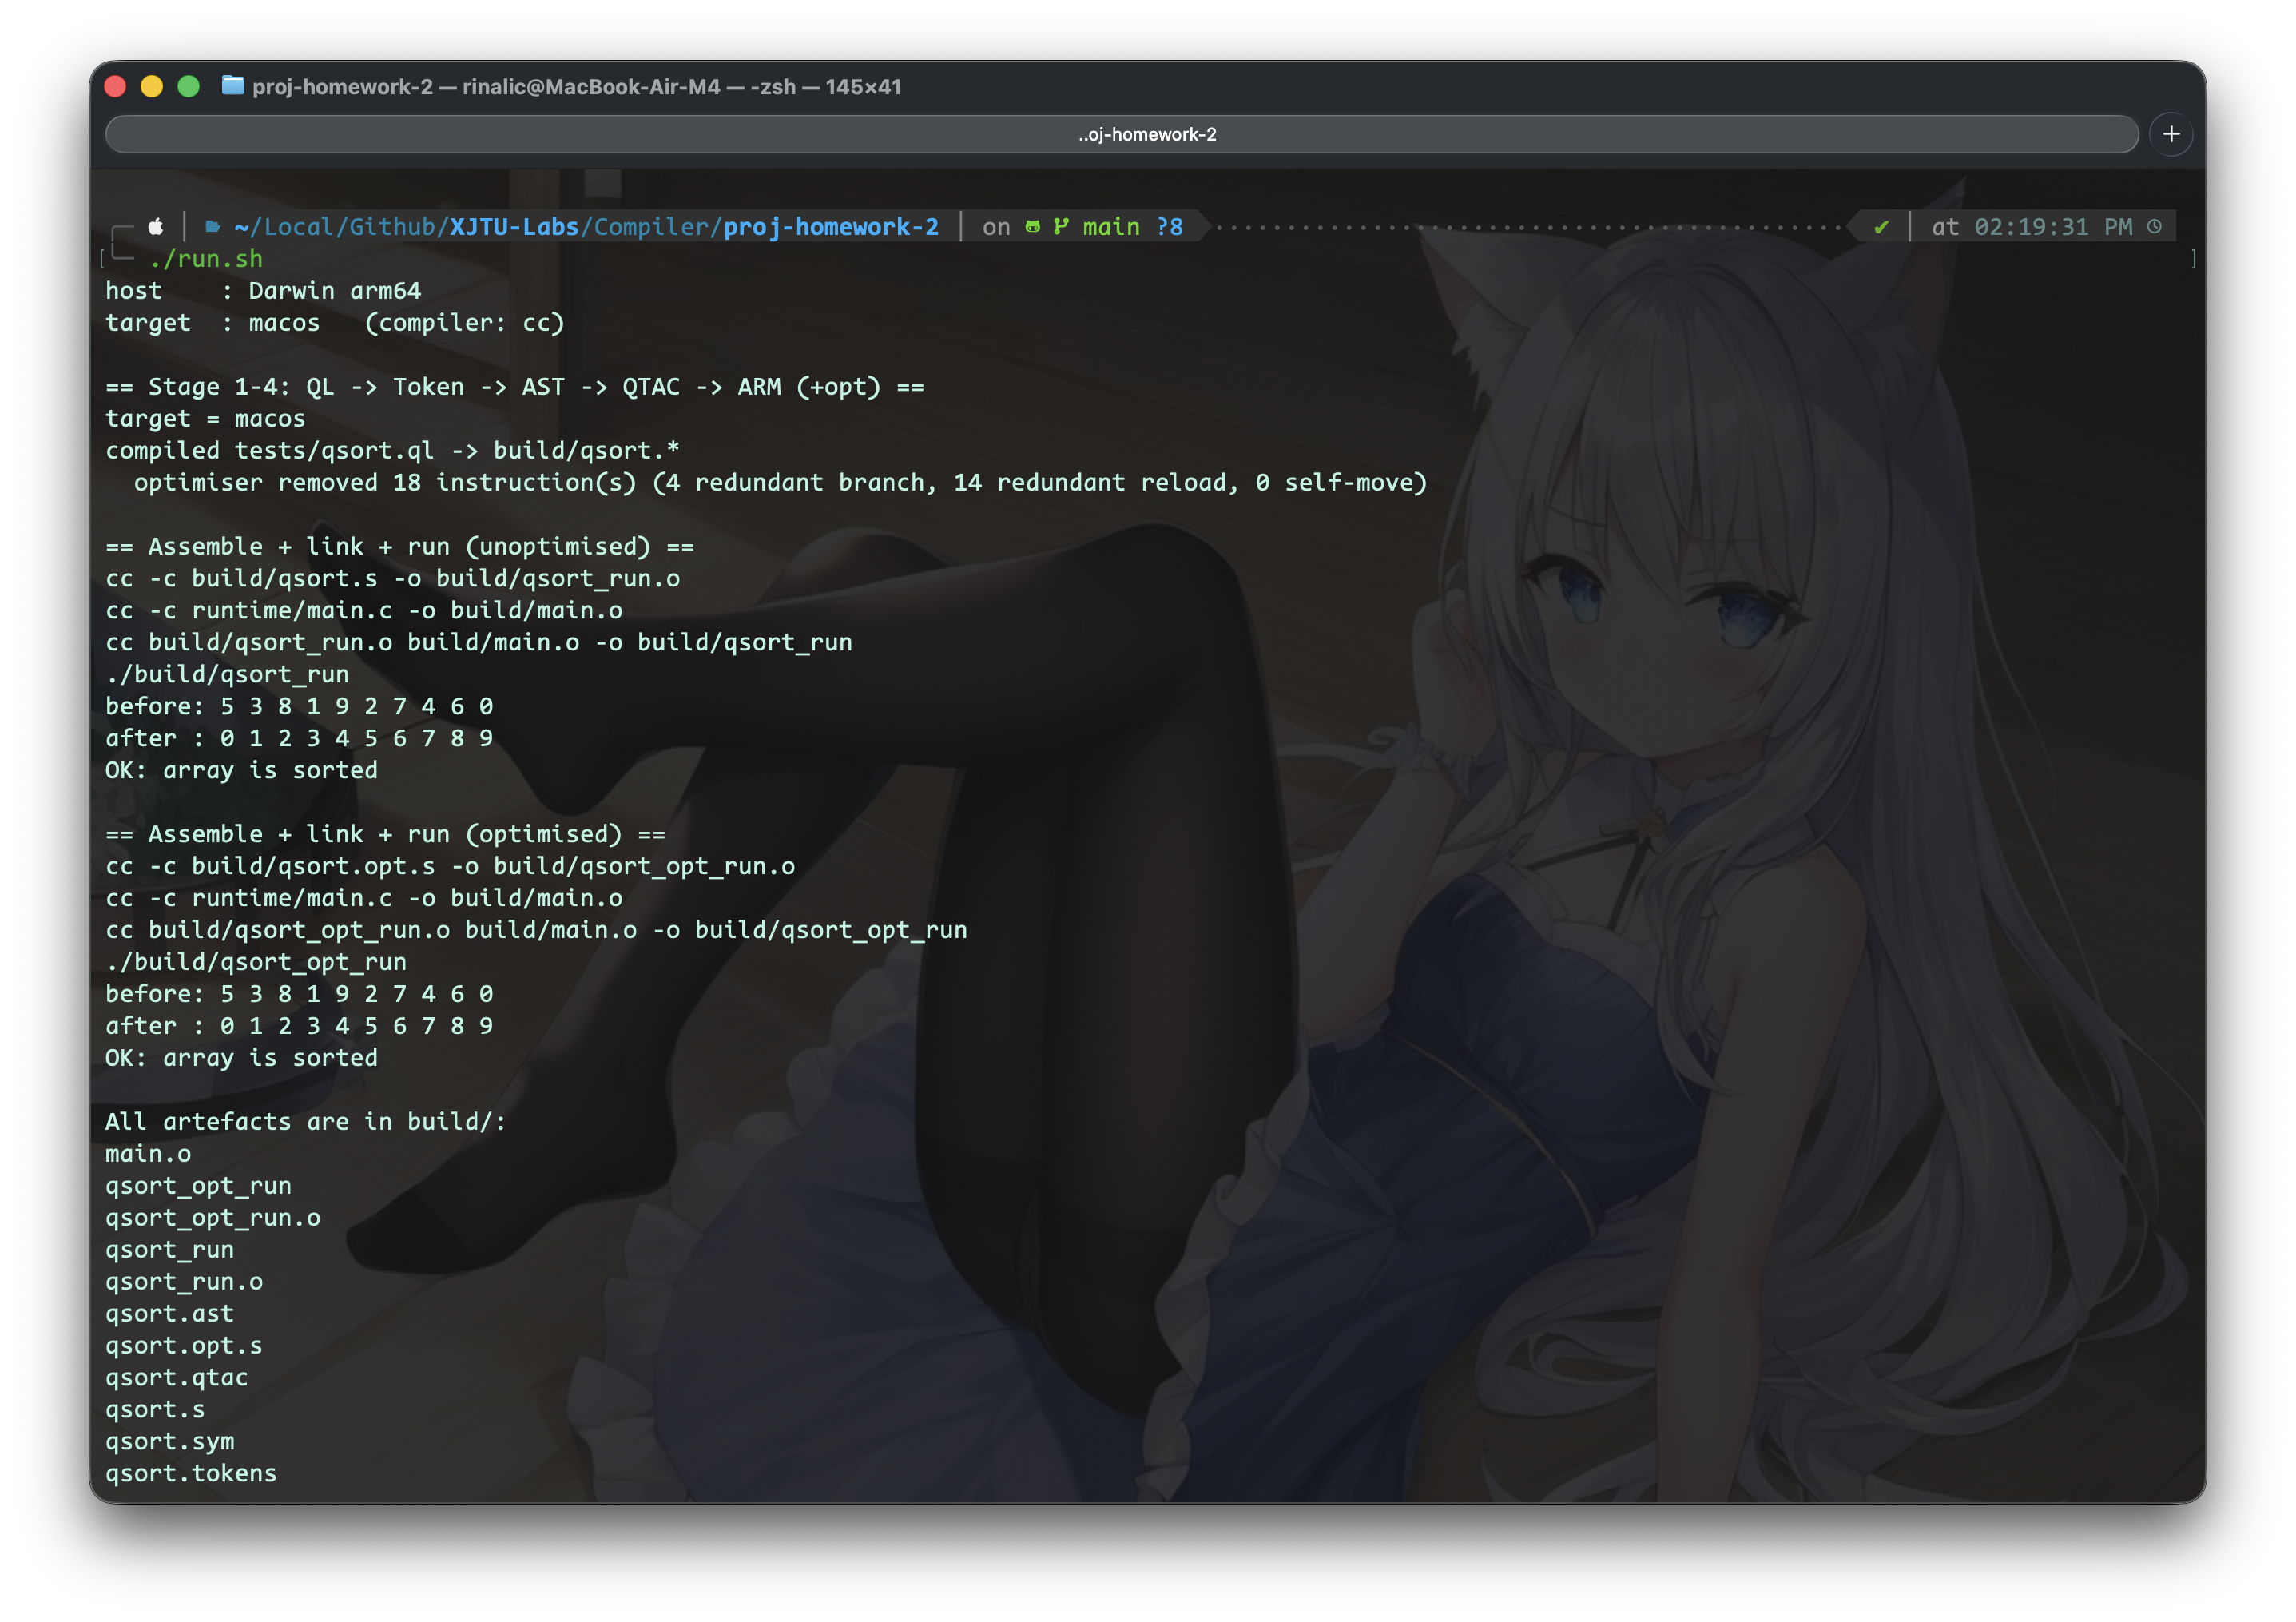
\includegraphics[width=0.95\textwidth]{images/run_result.png}
\caption{run.sh 完整运行结果（macOS arm64）}
\label{fig:run_result}
\end{figure}

截图中的关键信息逐行解读：

\begin{enumerate}
  \item \textbf{宿主信息}：\texttt{host: Darwin arm64}，\texttt{target: macos (compiler: cc)}——
        系统自动选择了 macOS 目标模式和 Apple Clang 编译器。

  \item \textbf{Stage 1-4 编译阶段}：\texttt{compiled tests/qsort.ql -> build/qsort.*}，
        说明词法、语法、QTAC、ARM 生成四个阶段均成功完成，并同时报告优化器删除了 18 条指令
        （4 条冗余跳转、14 条冗余加载、0 条自赋值）。

  \item \textbf{未优化版本运行结果}：
        \begin{itemize}
          \item \texttt{before: 5 3 8 1 9 2 7 4 6 0}——输入序列（随机乱序）
          \item \texttt{after : 0 1 2 3 4 5 6 7 8 9}——排序后的序列
          \item \texttt{OK: array is sorted}——正确性检验通过
        \end{itemize}

  \item \textbf{优化版本运行结果}：与未优化版本完全一致，同样输出
        \texttt{OK: array is sorted}，证明优化不改变程序语义。

  \item \textbf{生成的文件列表}：\texttt{build/} 目录下包含 \texttt{qsort.tokens}、
        \texttt{qsort.ast}、\texttt{qsort.qtac}、\texttt{qsort.sym}、\texttt{qsort.s}、
        \texttt{qsort.opt.s} 等全部交付物，以及汇编链接产生的目标文件和可执行文件。
\end{enumerate}

\subsection{各阶段输出统计}

\begin{table}[H]
\centering
\caption{各阶段输出文件统计}
\label{tab:outputs}
\begin{tabular}{llr}
\toprule
文件 & 内容 & 行数 \\
\midrule
\texttt{qsort.tokens} & Token 序列 & 235 \\
\texttt{qsort.ast}    & QAST 格式化输出 & 109 \\
\texttt{qsort.qtac}   & QTAC 三地址码 & 83 \\
\texttt{qsort.sym}    & 符号表 & 11 \\
\texttt{qsort.s}      & 未优化 ARM64 汇编 & 241 \\
\texttt{qsort.opt.s}  & 优化后 ARM64 汇编 & 223 \\
\bottomrule
\end{tabular}
\end{table}

\subsection{与参考 QTAC 对比分析}

\begin{table}[H]
\centering
\caption{本实现 QTAC 与材料参考 QTAC 的对比}
\label{tab:qtac_cmp}
\begin{tabular}{lll}
\toprule
方面 & 参考 QTAC & 本实现 QTAC \\
\midrule
全局声明 & \texttt{i80 a;} & \texttt{i80 a;}（一致） \\
函数结构 & \texttt{define f(a,b)\{...\}} & 一致 \\
标签命名 & \texttt{l0, l1, \ldots} & 一致 \\
临时变量命名 & \texttt{t0, t1, \ldots} & 一致 \\
数组寻址 & \texttt{t = arr + idx}（省略 $\times 8$） & \texttt{t = idx * 8; t = arr + t}（显式 $\times 8$） \\
条件跳转 & \texttt{IF q rop a THEN l ELSE l} & 一致 \\
函数调用 & \texttt{PAR a; \ldots; q = CALL f, k} & 一致 \\
顶层语句 & 直接列出（不封装函数） & 封装为 \texttt{define entry()\{\ldots\}} \\
\bottomrule
\end{tabular}
\end{table}

两者的结构性差异仅有两处：（1）字节偏移的显式计算（对正确运行必要）；（2）顶层语句的封装
方式（使代码生成器只需处理函数，无需特殊处理顶层代码）。控制流、命名约定和调用协议均与参
考完全一致。

% ============================================================
\section{总结}
% ============================================================

本实验成功实现了 QL 语言简易编译器 QCompiler 的完整路径 A（LL(1) 递归下降），覆盖编译原
理的全部核心阶段：

\begin{itemize}
  \item \textbf{词法分析}：正确识别 QL 的 5 类 Token，处理行注释和排版字符规范化，对
        \texttt{qsort.ql} 生成 235 个 Token。
  \item \textbf{语法分析与 AST 构建}：通过消除左递归、合并表达式/条件优先级梯级，实现了满
        足 LL(1) 条件的递归下降分析器，正确构建了完整的 QAST 树，所有结点类型均与 QASTNode
        规范对应。
  \item \textbf{QTAC 中间代码生成}：生成符合规范的 QTAC 三地址码和符号表，控制流结构、函
        数调用协议与参考 QTAC 高度一致，数组字节偏移显式计算确保代码可直接运行。
  \item \textbf{目标代码生成}：按 Q2ARM 指令模板将 QTAC 映射为 AAPCS64 兼容的 ARM64 汇
        编，采用全溢出策略，无需手工分配寄存器；同时支持 Linux/Kunpeng（\texttt{ADR}）和
        macOS（\texttt{ADRP/@PAGE}）两种全局地址化模式。
  \item \textbf{代码优化}：三遍窥孔优化删除 18 条冗余指令（约 7.5\%），优化前后运行结果完
        全一致。
  \item \textbf{端到端验证}：在 Apple Silicon macOS（arm64，与鲲鹏同架构）上一键运行，对
        10 元素整型数组成功执行快速排序并通过正确性检验。
\end{itemize}

\paragraph{主要经验}

本实验最具挑战性的环节是\textbf{文法变换}：QL 原始文法的二义性（$E$ 与 $C$ 混用导致括号
歧义）最终通过将两者合并为统一优先级梯级文法来解决，既消除了歧义，又避免了在 AST 中引入
多余的条件结点。另一个关键细节是\textbf{数组地址的字节偏移}：参考 QTAC 省略了 $\times 8$
的缩放，但在实际执行时必须显式计算，否则会访问错误的内存地址。

\paragraph{遗留问题}

本实现采用全溢出策略，寄存器利用率较低；完整的图着色寄存器分配将是进一步提升生成代码质量
的主要方向。此外，当前符号表对数组形参的类型记录较简单（仅记录 \texttt{int[]}），扩展为
携带维度信息后可支持多维数组。

% ============================================================
\section*{附录：实验源代码}
% ============================================================

\subsection*{A.1 词法分析器（lexer.py）}
\begin{lstlisting}[language=Python]
import re

KEYWORDS = {"int", "void", "if", "else", "while", "return"}
MULTI_OPS = ["<=", ">=", "==", "!=", "&&", "||", "+="]
SINGLE_OPS = set("+-*/=<>!")
DELIMS = set("(){}[];,")
GLYPH_FIX = {"x": "*", "-": "-", "-": "-", "-": "-"}

class Token:
    def __init__(self, type_, value, line, col):
        self.type = type_; self.value = value
        self.line = line;  self.col = col
    def __repr__(self): return f"({self.type}, {self.value})"

class LexError(Exception): pass

def normalise(text):
    for bad, good in GLYPH_FIX.items(): text = text.replace(bad, good)
    return text

def tokenize(text):
    text = normalise(text)
    tokens = []; line, col = 1, 1; i, n = 0, len(text)
    def adv(k=1):
        nonlocal i, col; i += k; col += k
    while i < n:
        c = text[i]
        if c == "\n": line += 1; col = 1; i += 1; continue
        if c in " \t\r": adv(); continue
        if c == "/" and i+1 < n and text[i+1] == "/":
            while i < n and text[i] != "\n": i += 1
            continue
        start_col = col
        if c.isdigit():
            m = re.match(r"[0-9]+", text[i:])
            tokens.append(Token("NUM", m.group(0), line, start_col))
            adv(len(m.group(0))); continue
        if c.isalpha() or c == "_":
            m = re.match(r"[a-zA-Z_][a-zA-Z0-9_]*", text[i:])
            word = m.group(0)
            ttype = "KEYWORD" if word in KEYWORDS else "ID"
            tokens.append(Token(ttype, word, line, start_col))
            adv(len(word)); continue
        two = text[i:i+2]
        if two in MULTI_OPS:
            tokens.append(Token("OP", two, line, start_col)); adv(2); continue
        if c in SINGLE_OPS:
            tokens.append(Token("OP", c, line, start_col)); adv(); continue
        if c in DELIMS:
            tokens.append(Token("DELIM", c, line, start_col)); adv(); continue
        raise LexError(f"illegal character {c!r} at line {line}, col {col}")
    tokens.append(Token("EOF", "$", line, col))
    return tokens

def dump_tokens(tokens):
    return "\n".join(f"({t.type}, {t.value})" for t in tokens if t.type != "EOF") + "\n"

if __name__ == "__main__":
    import sys
    sys.stdout.write(dump_tokens(tokenize(sys.stdin.read())))
\end{lstlisting}

\subsection*{A.2 LL(1) 递归下降分析器（parser\_ll1.py，节选）}
\begin{lstlisting}[language=Python]
import qast

class ParseError(Exception): pass

class Parser:
    def __init__(self, tokens): self.toks = tokens; self.pos = 0

    @property
    def cur(self): return self.toks[self.pos]
    def at(self, value): return self.cur.value == value
    def at_type(self, t): return self.cur.type == t
    def advance(self): t = self.cur; self.pos += 1; return t
    def expect(self, v):
        if self.cur.value != v:
            raise ParseError(f"line {self.cur.line}: expected {v!r} got {self.cur.value!r}")
        return self.advance()

    def parse_program(self):
        self.expect("{"); decls, stmts = self.parse_decls_and_stmts()
        self.expect("}"); return qast.Program(decls, stmts)

    def parse_decls_and_stmts(self):
        decls = []
        while self.cur.value in ("int", "void"): decls.append(self.parse_decl())
        stmts = []
        while not self.at("}"): stmts.append(self.parse_stmt())
        return decls, stmts

    def parse_decl(self):
        ret_type = self.advance().value
        name = self.expect_type("ID").value
        if self.at("("):
            params = self.parse_params()
            body = self.parse_block()
            return qast.FuncDecl(name, ret_type, params, body)
        dims = []
        if self.at("["):
            self.expect("["); dims.append(int(self.expect_type("NUM").value))
            self.expect("]")
        self.expect(";"); return qast.VarDecl(name, dims)

    def _left_assoc(self, sub, ops):
        node = sub()
        while self.cur.value in ops:
            op = self.advance().value; node = qast.Binary(op, node, sub())
        return node

    def parse_assign(self):
        left = self.parse_logic_or()
        if self.cur.value in ("=", "+="):
            op = self.advance().value; right = self.parse_assign()
            return qast.Binary(op, left, right)
        return left

    def parse_logic_or(self): return self._left_assoc(self.parse_logic_and, ("||",))
    def parse_logic_and(self): return self._left_assoc(self.parse_equality, ("&&",))
    def parse_equality(self): return self._left_assoc(self.parse_relational, ("==","!="))
    def parse_relational(self): return self._left_assoc(self.parse_additive, ("<","<=",">",">="))
    def parse_additive(self): return self._left_assoc(self.parse_mul, ("+","-"))
    def parse_mul(self): return self._left_assoc(self.parse_unary, ("*","/"))

    def parse_postfix(self):
        node = self.parse_primary()
        while self.at("["):
            self.expect("[")
            if self.at("]"): self.expect("]")   # arr[] 退化形式
            else:
                idx = self.parse_expr(); self.expect("]")
                node = qast.Index(node, idx)
        return node

def parse(tokens): return Parser(tokens).parse_program()
\end{lstlisting}

\subsection*{A.3 QTAC 生成器（irgen.py，节选）}
\begin{lstlisting}[language=Python]
WORD = 8

class IRGen:
    def __init__(self):
        self.code = []; self.tcount = 0; self.lcount = 0
        self.globals = {}; self.scope = {}; self.symtab_lines = []

    def new_temp(self): t = f"t{self.tcount}"; self.tcount += 1; return t
    def new_label(self): l = f"l{self.lcount}"; self.lcount += 1; return l
    def emit(self, s): self.code.append(s)

    def gen_addr(self, e):
        # 数组元素地址 = base + index * 8
        base = self.gen_expr(e.base); idx = self.gen_expr(e.index)
        idx = self._as_register(idx)
        off = self.new_temp(); self.emit(f"{off} = {idx} * {WORD}")
        addr = self.new_temp(); self.emit(f"{addr} = {base} + {off}")
        return addr

    def gen_cond(self, c, l_true, l_false):
        if c.kind == "Binary" and c.op in self.REL:
            a = self.gen_expr(c.left); b = self.gen_expr(c.right)
            a = self._as_register(a)
            self.emit(f"IF {a} {c.op} {b} THEN {l_true} ELSE {l_false}")
        elif c.kind == "Binary" and c.op == "&&":
            mid = self.new_label()
            self.gen_cond(c.left, mid, l_false)
            self.emit(f"LABEL {mid}")
            self.gen_cond(c.right, l_true, l_false)
        elif c.kind == "Unary" and c.op == "!":
            self.gen_cond(c.operand, l_false, l_true)  # 交换真假标签
\end{lstlisting}

\subsection*{A.4 窥孔优化器（optimize.py）}
\begin{lstlisting}[language=Python]
import re

def optimize(asm_text):
    lines = asm_text.splitlines()
    stats = {"branches": 0, "reloads": 0, "selfmoves": 0, "removed": 0}

    # 遍 1：冗余跳转（B Lx 紧接 Lx:）
    out = []; i = 0
    while i < len(lines):
        m = re.match(r"^\s*B\s+(\w+)$", lines[i])
        if m and i+1 < len(lines) and lines[i+1].strip() == f"{m.group(1)}:":
            stats["branches"] += 1; i += 1; continue
        out.append(lines[i]); i += 1
    lines = out

    # 遍 2：STR Xr,[sp,#k] 紧接 LDR Xr,[sp,#k] -> 删除 LDR
    str_re = re.compile(r"^\s*STR\s+(X\w+),\s*\[sp, #(\d+)\]$")
    ldr_re = re.compile(r"^\s*LDR\s+(X\w+),\s*\[sp, #(\d+)\]$")
    out = []; i = 0
    while i < len(lines):
        s = str_re.match(lines[i])
        l2 = ldr_re.match(lines[i+1]) if i+1 < len(lines) else None
        if s and l2 and s.group(1)==l2.group(1) and s.group(2)==l2.group(2):
            out.append(lines[i]); stats["reloads"] += 1; i += 2; continue
        out.append(lines[i]); i += 1
    lines = out

    # 遍 3：MOV Xr, Xr -> 删除
    out = []
    for line in lines:
        m = re.match(r"^\s*MOV\s+(X\w+),\s*(X\w+)$", line)
        if m and m.group(1) == m.group(2): stats["selfmoves"] += 1; continue
        out.append(line)
    stats["removed"] = stats["branches"]+stats["reloads"]+stats["selfmoves"]
    return "\n".join(out)+"\n", stats
\end{lstlisting}

\subsection*{A.5 运行命令}
\begin{verbatim}
# 一键端到端测试（自动检测平台）
./run.sh

# 手动运行各阶段（以 macOS 为例）
python3 src/lexer.py       < tests/qsort.ql         # 输出 Token 流
python3 src/parser_ll1.py  < tests/qsort.ql         # 输出 QAST
python3 src/irgen.py       < tests/qsort.ql         # 输出 QTAC
python3 src/codegen.py --macos < build/qsort.qtac   # 输出 ARM64（macOS）

# 完整编译（生成全部中间文件）
python3 src/qcc.py tests/qsort.ql -o build --target macos

# 汇编 + 链接 + 运行（macOS）
cc -c build/qsort.s  -o build/qsort.o
cc -c runtime/main.c -o build/main.o
cc build/qsort.o build/main.o -o build/qsort_run
./build/qsort_run

# 鲲鹏/Linux 平台（--target linux 为默认值）
python3 src/qcc.py tests/qsort.ql -o build
gcc -c build/qsort.s  -o build/qsort.o
gcc -c runtime/main.c -o build/main.o
gcc build/qsort.o build/main.o -o build/qsort_run
./build/qsort_run
\end{verbatim}

\end{document}
